%!TEX root = ../../main.tex

\begin{figure}[tp]
  \centering
  \footnotesize

  \caption{QQ Plots of Standardized Residuals of ARMA-GARCH Models}

  \begin{longcaption}
    Empirical and theoretical standardized residuals from the best (lowest BIC) ARMA-GARCH model specifications using normal, symmetric \emph{t} and skewed \emph{t} innovations. Data from the theoretical distribution should line up on the dashed line. Based on weekly data 1963--2016.
  \end{longcaption}

  \begin{subfigure}{0.70\textwidth}
    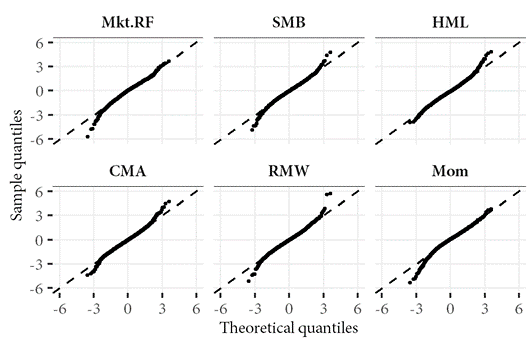
\includegraphics[width=\textwidth]{graphics/qq_norm.png}
    \caption{Normal}
  \end{subfigure}
  \begin{subfigure}{0.70\textwidth}
    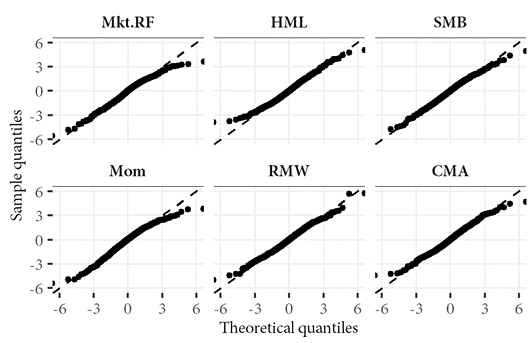
\includegraphics[width=\textwidth]{graphics/qq_std.png}
    \caption{Student's \textit{t}}
  \end{subfigure}
  \begin{subfigure}{0.70\textwidth}
    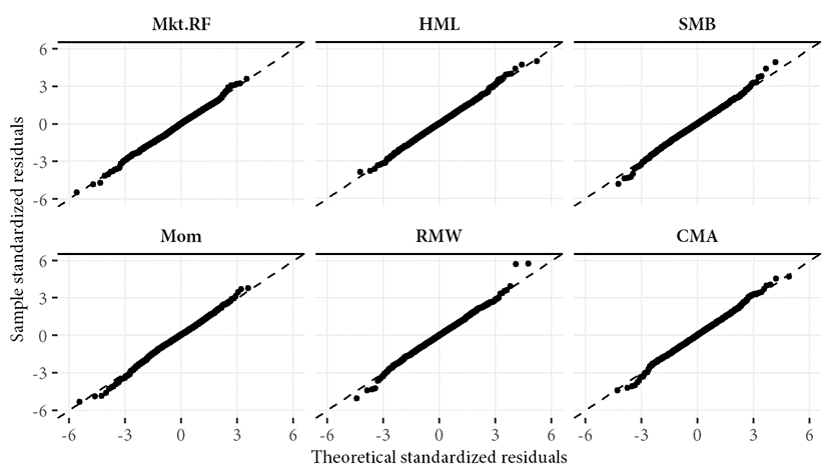
\includegraphics[width=\textwidth]{graphics/qq_ghst.png}
    \caption{Skewed Student's \textit{t}}
  \end{subfigure}

  \label{fig:garch_qq}
\end{figure}
